\documentclass{bmvc2k}
\RequirePackage[table]{xcolor}% for colored tabular rows
\usepackage{times}
\usepackage{epsfig}
\usepackage{graphicx}
\usepackage{amsmath}
\usepackage{amssymb}
\usepackage{subfigure}
\usepackage{multirow}
%% Enter your paper number here for the review copyu
%\bmvcreviewcopy{460}



%%%%%%%%%%%%%%%%%%%%%%%%%%%%%%%%%%
% AZ's macros
%%%%%%%%%%%%%%%%%%%%%%%%%%%%%%%%%%
% Stuff for doing vector.
\def\vec#1{\mathchoice%
        {\mbox{\boldmath $\displaystyle\bf#1$}}
        {\mbox{\boldmath $\textstyle\bf#1$}}
        {\mbox{\boldmath $\scriptstyle\bf#1$}}
        {\mbox{\boldmath $\scriptscriptstyle\bf#1$}}}
\def\v#1{\protect\vec #1}


% Stuff for doing matrix.
\def\mat#1{\mathchoice{\mbox{\boldmath$\displaystyle\tt#1$}}
        {\mbox{\boldmath$\textstyle\tt#1$}}
        {\mbox{\boldmath$\scriptstyle\tt#1$}}
        {\mbox{\boldmath$\scriptscriptstyle\tt#1$}}}
\def\m#1{\protect\mat #1}

\newcommand{\matx}[1]{{\m #1}}

\newcommand{\tr}{\mbox{$^{\top}$}}
\newcommand{\mtr}{\mbox{$^{-\top}$}}



%\title{Author Guidelines for the\\ British Machine Vision Conference}
%\title{Recognizing human actions in still images: a dataset, baselines and performance evaluation }
%\title{Recognizing human actions in still images: \\ comparison of bag-of-features and part-based approaches }
%\title{Recognizing human actions in still images: \\ a comparison of bag-of-features and part-based approaches }
%\title{Recognizing human actions in still images: \\ a comparison of bag-of-features and part-based representations}
\title{Recognizing human actions in still images: \\ a study of bag-of-features and part-based representations}
%\title{Recognizing human actions in still images: \\  bag-of-features or\\ part-based representation?}
%\title{Comparison of structured and unstructured representations for recognizing human actions in still images}

%\title{Recognizing human actions in still images: \\ a comparative study of bag-of-features and part-based approaches. }
%\title{Bag-of-features models for classification of human actions in still images}



% Enter the paper's authors in order
% \addauthor{Name}{email/homepage}{INSTITUTION_CODE}
\addauthor{Vincent Delaitre}{vincent.delaitre@ens-lyon.org}{1}
%\addauthor{Vincent Delaitre}{vincent.delaitre@ens-lyon.org}{1}
\addauthor{Ivan Laptev}{ivan.laptev@inria.fr}{2}
\addauthor{Josef Sivic}{josef.sivic@ens.fr}{2}

% Enter the institutions
% \addinstitu	tion{Name\\Address}
\addinstitution{
\'Ecole Normale Sup\'erieure de Lyon
}
%\addinstitution{
%Willow Project\\
%\'Ecole Normale Sup\'erieure\\
%CNRS/ENS/INRIA (UMR 8548)\\
%}

\addinstitution{
INRIA - Willow Project\\
%Laboratoire d'Informatique de l'Ecole Normale Superieure\\
Laboratoire d'Informatique\\
\'Ecole Normale Sup\'erieure\\
CNRS/ENS/INRIA (UMR 8548)\\
}

\runninghead{Delaitre, Laptev, Sivic}{Recognizing human actions in still images.}

% Any macro definitions you would like to include
% These are not defined in the style file, because they don't begin
% with \bmva, so they might conflict with the user's own macros.
% The \bmvaOneDot macro adds a full stop unless there is one in the
% text already.
\def\eg{\emph{e.g}\bmvaOneDot}
\def\Eg{\emph{E.g}\bmvaOneDot}
\def\etal{\emph{et al}\bmvaOneDot}

\newcommand{\red}[1]{{\em \small \color{red} #1}} % add
\definecolor{mygreen}{rgb}{0.0,0.6,0.1}
%\newcommand{\green}[1]{{\color{mygreen} #1}} %added
\newcommand{\green}[1]{#1} %added

\newcommand{\ok}[1]{{\small \scriptsize  \color{mygreen} #1}} %added
\newcommand{\bad}[1]{{\small \scriptsize  \color{red} #1}} %added


\newcommand{\secnspc}{\vspace*{-3mm}}       % -3
\newcommand{\subsecnspc}{\vspace*{-1.4mm}}  % -1.4
\newcommand{\parnspc}{\vspace*{-4.2mm}}     % -4.2
\newcommand{\capnspc}{\vspace*{-4mm}}       % -4
\newcommand{\tablespc}{\vspace{-4mm}}

\newcommand{\tfs}{\small}   % tabular font size
\newcommand{\cfs}{\small}   % caption font size


%------------------------------------------------------------------------- 
% Document starts here
\begin{document}



\maketitle

\begin{abstract}
Recognition of human actions is usually addressed in the scope of video
interpretation.
Meanwhile, common human actions such as ``reading a book'', ``playing a guitar''
or ``writing notes'' also provide a natural description for many still images.
In addition, some actions in video such as ``taking a photograph'' are static by their
nature and may require recognition methods based on static cues only.
Motivated by the potential impact of recognizing actions in still images
and the little attention this problem has received in computer vision
so far, we address recognition of human actions in
consumer photographs.
We construct a new dataset with seven classes of actions in 968 Flickr images
representing natural variations
of human actions in terms of camera view-point, human pose, clothing, occlusions and scene background.
We study action recognition in still images using the state-of-the-art bag-of-features methods as well
as their combination with the part-based Latent SVM approach of Felzenszwalb~\etal~\cite{Felzenszwalb09}.
In particular, we investigate the role of background scene context and demonstrate
that improved action recognition performance can be achieved by
 (i) combining the statistical and part-based representations,
 and (ii) integrating person-centric description with the background scene context. 
%We show results on our newly collected dataset of seven common actions
%as well as  demonstrate improved performance over existing methods on the sports dataset of person-object interactions by Gupta~\etal~\cite{Gupta09}.
We show results on our newly collected dataset of seven common actions
as well as  demonstrate improved performance over existing methods on the datasets of Gupta~\etal~\cite{Gupta09}
and Yao and Fei Fei~\cite{FeiFei10a}.
%
%Recognition of human actions is usually addressed in the scope of video
%interpretation.
%Meanwhile, common human actions such as ``reading a book'', ``playing a guitar''
%or ``writing notes'' also provide a natural description for many still images.
%In addition, some actions in video such as ``taking a photograph'' are static by their
%nature and may require recognition methods based on static cues only.
%Motivated by the potential impact of recognizing actions in still images
%and the little attention this problem has received in computer vision
%so far, we address recognition of human actions in
%consumer photographs.
%We construct a new dataset with seven classes of actions in 968 Flickr images
%representing natural variations
%of human actions in terms of camera view-point, human pose, clothing, occlusions and scene background.
%We study action recognition in still images using state-of-the-art statistical methods as well
%as their combination with the part-based Latent SVM approach of Felzenszwalb~\etal~\cite{Felzenszwalb09}.
%In particular, we investigate the role of background scene context and demonstrate
%that improved action recognition performance can be achieved by
% (i) combining the statistical and part-based representations,
% and (ii) integrating person-centric description with the background scene context. 
%We show results on our newly collected dataset of seven everyday actions
%and  demonstrate improved performance over existing methods on the dataset of person-object interactions in sports of Gupta~\etal~\cite{Gupta09}.
%
%While action recognition in video has recently received significant attention, action recognition
%in still images is relatively unexplored domain. 
%%- We address the problem of action recognition in still images.
%Following contributions:
%- investigate the bof representation on the problem.  
%Experimentally compare a range of parameters including kernels, and different ways of including background information and show that representation combining of person centric description and image level description on the kernel level performs best. \\
%- further show that combining with structured discriminatively trained flexible part based person centric representation of Felzenswalb et al. further improves performance. \\
%- collect new dataset of real Flickr images containing common everyday actions  not focused on a particular domain such as  sports.\\
%- Show results on the newly collected dataset. outperform the approach of Gupta on his own dataset. 
% and the dataset of sports of Gupta, where we outperform the current state-of-the-art.
%- show that combination of LSVM and BOF is doing best\\
%- cf. results with Gupta on his own data and improve performance. \\

\end{abstract}

%%%%%%%%%%%%%%%%%%%%%%%%
\secnspc
\section{Introduction}
\secnspc

%%%%%%%%%%%%%%%%%%%%%%%%
\label{sec:intro}



\begin{figure}[tbp]
%\centering
 \small
%\includegraphics[height=.5\linewidth]{figs/dataset.pdf}
%\includegraphics[height=.5\linewidth]{figs/images.png}
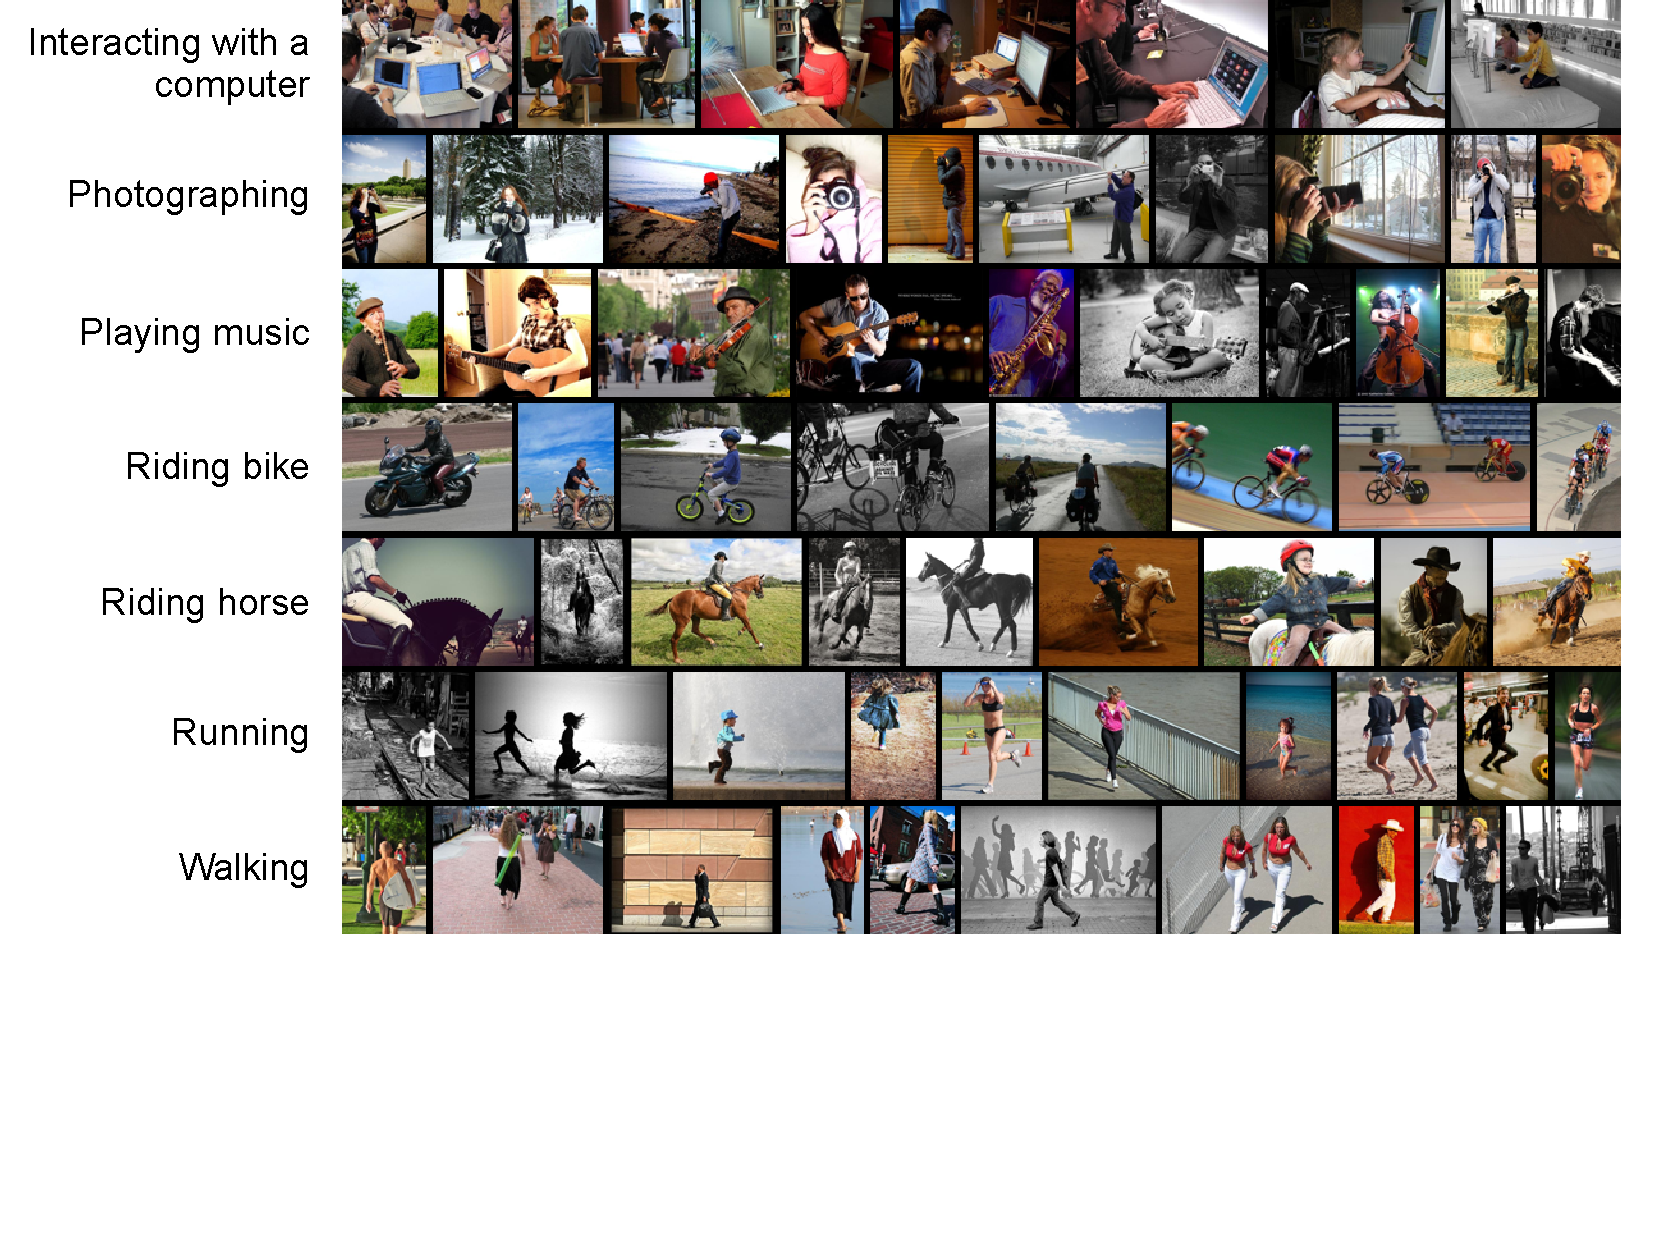
\includegraphics[width=.95\linewidth]{figs/my_dataset_cropped.pdf}
\capnspc
\caption{\cfs Example images from our new dataset with seven human action classes collected from Flickr.
Note the natural and challenging variations in the camera view-point, clothing of people, occlusions, object appearance and scene layout present in the consumer photographs.
%The manually annotated bounding boxes indicating the location of the person performing the action are overlaid in yellow. 
 %\red{*** Replace these Gupta images with examples of our images. Make images slightly bigger.}
 \normalsize
   }
 \label{fig:dataset}
\capnspc
\end{figure}


Human actions represent essential content of many images. Recognizing human actions in still images will potentially provide useful meta-data to many applications such as indexing and search of large-scale image archives. Given the frequent interactions of people with objects (e.g. ``answer phone'') and scenes (e.g. ``walking around the corner''), human action recognition is also expected to help solving other related problems for still images such as object recognition or  scene layout estimation.

Recognition of human actions has mostly been explored in video, see for example~\cite{BoDa01,Laptev08,MHK06}. While the motion of people often provides discriminative cues for action classification, many actions such as the ones illustrated in Figure~\ref{fig:dataset} can be identified from single images. Moreover, several types of actions such as ``taking a photograph'' and ``reading a book'' are of static nature and may require recognition methods based on static cues only even if the video is available.

%The goal of this work is to study recognition of common human actions represented in typical still images such as consumer photographs. This problem has received little attention in the past with the exception of a few related
%papers~\cite{Gupta09,Ikizler09,Ikizler08,Li07,Wang06}. 
The goal of this work is to study recognition of common human actions represented in typical still images such as consumer photographs. This problem has received little attention in the past with the exception of few related
papers focused on specific domains, such as sports actions~\cite{Gupta09,Ikizler08,Li07,Wang06} or, more recently, people playing musical instruments~\cite{FeiFei10a}. Learning from still images to recognize actions in video was investigated in~\cite{Ikizler09}. 

The proposed methods~\cite{Gupta09,Ikizler08,Wang06} have mainly relied on the body pose as a cue for action recognition. While promising results have been demonstrated on sports actions~\cite{Gupta09,Ikizler08,Wang06}, typical action images such as the ones illustrated in Figure~\ref{fig:dataset} often contain heavy occlusions and significant changes in camera viewpoint causing serious challenges for current body-pose estimation methods. At the same time, the presence of particular objects~\cite{Gupta09} and scene types~\cite{Li07} often characterizes the action and can be used for action recognition.

To deal with various types of actions in still images, we avoid explicit reasoning about body poses and investigate more general classification methods. We study action recognition in typical consumer photographs and construct a new dataset with seven classes of actions in 968 images obtained from Flickr photo-sharing website. Image samples in Figure~\ref{fig:dataset} illustrate the natural and challenging variations of actions in our dataset with respect to camera view-points, clothing of people, occlusions, object appearance and scene layout.

We study performance of statistical bag-of-features representations combined with SVM classification~\cite{Zhang07}. In particular, we investigate person-centric representations and study the influence of background/context information on action recognition. We investigate a large set of parameters on the validation set and show a consistent generalization of results to the test set. In addition to statistical methods, we investigate the structural part-based  LSVM model of Felzenszwalb~\etal~\cite{Felzenszwalb09} and demonstrate improved performance of their combination. Based on the comparative evaluation on the datasets of~\cite{Gupta09} and~\cite{FeiFei10a} we demonstrate that previous methods relying on explicit body-pose estimation can be significantly outperformed by more generic recognition methods investigated in this paper.

The rest of the paper is organized as follows. In Section~\ref{sec:dataset} we describe our new dataset for action recognition in still images and detail performance measures used in our evaluation. Sections~\ref{sec:bof} and~\ref{sec:lsvm} present the two recognition methods investigated in this paper and their combination. Section~\ref{sec:results} provides experimental evaluation of alternative methods and corresponding parameter settings on the three still-image action datasets. %Section~\ref{sec:conclusion} concludes the paper.

%\begin{itemize}

%\item The problem: action recognition in still images.

%\item Differences from actions in video.

%\item Why is it difficult?

%\item Related work: 
%\begin{itemize}
% \item actions in video.
% \item Actions in still images: not much work. Aggarwal. Nazli. Fei-Fei in CVPR 2010.\\
% Here the goal is to: (1) provide a difficult dataset of realistic actions, not focused on one domain as in previous work (sports in Aggarwal or playing instruments in Fei-Fei). (2) Evaluate state-of-the-art baselines for classification and detection. 
% 
% \item {BoF} models for image classification. Also state-of-the-art in action classification in video (Laptev et al.)
% \item Structured representations for object detection.
%\end{itemize}
%  
%\end{itemize}



%%%%%%%%%%%%%%%%%%%%%%%%
\secnspc
\section{Datasets and performance measures}
\secnspc
%%%%%%%%%%%%%%%%%%%%%%%%
\label{sec:dataset}

%We consider three datasets in this work: the person-object interactions dataset collected by Gupta~\etal~\cite{Gupta09} and our newly collected dataset of actions in consumer photographs. 
%%We test the compared methods on the dataset of sports person-object interactions collected by Gupta~\etal~\cite{Gupta09} and our newly collected dataset of actions in still images. 
%The dataset of~\cite{Gupta09} is focused on sports and contains 50 images for each of the following six actions: ``Cricket defensive shot", ``Cricket bowling", ``Croquet shot", ``Tennis serve", ``Volleyball smash" and ``Tennis Forehand".   In addition, images are centred  on the person and cropped to eliminate the background.  

We consider three datasets in this work:  the datasets of Gupta~\etal~\cite{Gupta09} and Yao and Fei Fei~\cite{FeiFei10a}, focused on sports and people playing musical instruments, respectively,  as well as  our newly collected dataset of actions in consumer photographs.  To avoid the focus on specific domains and to investigate the effect of the background (images in~\cite{Gupta09,FeiFei10a} were cropped to eliminate the background) we collect a new dataset of original consumer photographs depicting seven common human actions: ``Interacting with computers", ``Photographing", ``Playing a musical instrument", ``Riding bike", ``Riding horse", ``Running" and ``Walking".  Images for the \green{"Riding bike"} action were taken from the Pascal 2007 VOC Challenge and the remaining images were collected from Flickr by querying on keywords such as \green{``running people" or ``playing piano"}.  Images clearly not depicting the action of interest were manually removed. In this way we have collected a total of  968 photographs -- \green{at least 108} images for each class, split into \green{70 images per class} for training and \green{the remaining ones} for test. Each image was manually annotated with bounding boxes indicating the locations of people. % of the  person. 
For these annotations we have followed Pascal VOC guidelines. \green{In particular, we have labeled each person with a bounding box being the smallest rectangle containing its visible pixels. 
%The bounding boxes are labelled as 'Truncated' if more than 15\%-20\% of the person is occluded or lies outside the bounding box. 
We have also added a field  ``action" to each bounding box to describe which action(s) are executed.} % (note that there can be multiple actions for a single person).}
Example images for each of the seven classes are shown in figure~\ref{fig:dataset}.
%We plan to make our dataset together with the person annotations publicly available. %\red{What about images with a copyright?}

\parnspc
\paragraph{Performance measures:}

We use two performance measures throughout the paper: (i) the {\em classification accuracy} and  (ii) the {\em mean average precision (mAP)}. The classification accuracy is obtained as the average of the diagonal of the confusion table between different classes, and is  a typical performance measure for multi-way classification tasks.
To obtain mAP we first compute the area under precision-recall curve (average precision) for each of the seven binary 1-vs-all action classifiers. mAP is then obtained as the mean of average precisions across seven action classes.
% The mAP is obtained as the mean of average precisions (the area under the precision-recall curve)  over  of the seven binary 1-vs-all action classifiers. mAP is then obtained as the mean of the average precision across the seven action classes.

%The performance of this multi-way classification task is measured by a confusion table, which indicates percentage of correctly classified images for each class and the level of confusion between different classes. As a single number measure of the accuracy we use the average of the diagonal of the confusion table. 

%\red{Josef: We also report MAP, add MAP description, add MAP to table 1a. and LSVM results.}

% random samples of consumer photographs. We have not constrained them in any sense.
%Hence wide variation of camera viewpoint and some variation of persons pose.
% varied backgrounds

%%%%%%%%%%%%%%%%%%%%%%%%
\secnspc
\section{Bag-of-features classifier}
\secnspc
%%%%%%%%%%%%%%%%%%%%%%%%
\label{sec:bof}

Here we describe the spatial pyramid bag-of-features representation~\cite{Lazebnik06} 
with the Support Vector Machine (SVM) classifier~\cite{Scholkopf} and the implementation choices investigated in this work.  In particular, we provide details for the used image representations and SVM classifier kernels as well as for
different methods of integrating information on the person bounding boxes and the scene background into the classifier. 
%In particular we examine performance with respect to (i) vocabulary size, (ii)  spatial pyramid binning, (iii) different kernels for the SVM classifier, and (iv) different ways of incorporating the person bounding box into the classifier. 


%Here we describe the experiments performed with the spatial pyramid bag-of-features representation~\cite{Lazebnik06} 
%using a Support Vector Machine (SVM) classifier~\cite{Scholkopf}.  In particular we test performance with respect to (i) vocabulary size, (ii)  spatial pyramid binning, (iii) different kernels for the SVM classifier, and (iv) different ways of incorporating the person bounding box into the classifier. 
%The performance is tested for the three different setups (Cropped, Original and BBox) described in section~\ref{}. Finally, in the BBox setup, we also experiment with different ways of incorporating the person bounding box information into the classifier. 

\parnspc
\paragraph{Image representation:}
Images (or image regions given by a rectangular bounding box) are represented using SIFT descriptors sampled on \green{10 regular grids with increasing scales with spacing $s_i = \lfloor12 \cdot 1.2^i\rfloor$ pixels for $i = 0, \cdots, 9$. The scale of features extracted from each grid is set to $w_i = 0.2 \cdot s_i$.}
 Visual vocabularies are built from training descriptors  using k-means clustering. We consider vocabularies of sizes $K\in\{256, 512, 1024, 2048, 4096\}$ visual words. Descriptors from both training and test sets are then assigned to one of the visual words
 and aggregated into a $K$-dimensional histogram, denoted further as the bag-of-features representation.
  Following the spatial pyramid representation of Lazebnik~\etal~\cite{Lazebnik06} we further divide the image into  $1\times1$ (Level 0), $2\times2$ (Level 1) and $4\times4$ (Level 2)  spatial grids of cells. Local histograms within  each cell are then concatenated with weights 0.25, 0.25 and 0.5 for levels 0, 1, and 2, respectively. This results in a $(1 + 4 + 16)K=21K$ dimensional representation, where $K$ is the vocabulary size. The weights of different histogram levels are kept fixed throughout the experiments, but could be potentially learnt as shown in~\cite{Bosch07}. This representation captures a coarse spatial layout of the image (or an image region) and is often beneficial for scene classification in still images~\cite{Lazebnik06} and action classification in videos~\cite{Laptev08}.

\parnspc
\paragraph{Support vector machine classification:}
%For classification we use the SVM classifier. 
Classification is performed with
the SVM classifier using the 1-vs-all scheme, which, in our experiments, resulted in a small but consistent improvement
over the 1-vs-1 scheme. 
%In the following, we denote by $K(a,b)$ the kernel value between visual word histograms $ a$ and $ b$ of  two different images. 
%In the following, $\v x$ and $\v y$ denote visual word histograms of images $X$, $Y$. 
%We experiment with four different kernels: \\
%(i) the histogram intersection kernel, given by $\sum_i \min(a_i,b_i)$; \\
%(ii) the $\chi^2$ kernel, given by $\exp\{\frac{1}{\gamma} \sum_i \frac{(a_i-b_i)^2}{a_i+b_i}\}$; \\ 
%(iii)  the Radial basis function (RBF) kernel $\exp\{\frac{1}{\beta} \sum_i (a_i-b_i)^2\}$; and \\
%(iv) the linear kernel given by $\sum_i a_i b_i$. \\
We investigate four different kernels: 
\begin{enumerate}
\item the histogram intersection kernel, given by $\sum_i \min(x_i,y_i)$;
\item the $\chi^2$ kernel, given by $\exp\{-\frac{1}{\gamma} \sum_i \frac{(x_i-y_i)^2}{x_i+y_i}\}$; 
\item  the Radial basis function (RBF) kernel, given by  $\exp\{-\frac{1}{\beta} \sum_i (x_i-y_i)^2\}$; and
\item the linear kernel given by $\sum_i x_i y_i$.
\end{enumerate}
 $\v x$ and $\v y$ denote visual word histograms, and $\gamma$ and $\beta$ are
kernel parameters.
For the $\chi^2$ and intersection kernels, histograms are normalized to have unit L1 norm.
For the RBF and linear kernels, histograms are normalized to have unit L2 norm~\cite{Vedaldi09}.
Parameters $\gamma$ and $\beta$ of the $\chi^2$ and RBF kernels, respectively, 
together with the regularization parameter of the SVM are set for each experiment by a 5-fold cross validation
on the training set.

\parnspc
\paragraph{Incorporating the person bounding box into the classifier:}

%\paragraph{Experimental setups:}
Previous work on object classification~\cite{Zhang07} demonstrated that background is often correlated
with objects in the image (e.g.\ cars often appear on streets) and can provide useful signal for the classifier.
The goal here is to investigate different ways of incorporating the background information into the classifier for actions in still images.
%We consider different ways of incorporating the manually provided person bounding box into classification:   
%We also consider three experimental setups: 
We consider the following four approaches:
\begin{enumerate}
\item[A.] {\bf ``Person":}  Images are centred on the bounding of the person performing the action, cropped to contain $1.5\times$ the size of the bounding box, and re-sized such that the larger dimension is 300 pixels. This setup is similar to that of Gupta~\etal~\cite{Gupta09}, i.e. the person occupies the majority of the image and the background is largely suppressed.

\item[B.] {\bf ``Image":} Original images are resized to have the larger dimension at most 500 pixels. 
%\red{It would be more correct to say: "Images with the larger dimension bigger than 500 pixels are rescaled to fit in this limit."} 
No cropping is performed. The person bounding box is not used in any stage of training or testing apart from evaluating the performance. Here the visual word histograms represent a mix of the action and the background.

\item[C1.] {\bf ``Person+Background':} Original images are resized so that the maximum dimension of the $1.5\times$ rescaled person bounding box is 300 pixels, but no cropping is performed. The $1.5\times$ rescaled person bounding box is then used in both training and test to localize the person in the image and to provide a coarse segmentation of the image into foreground (inside the rescaled person bounding box) and background (the rest of the image). 
The foreground and background regions are treated separately. %represented using two separate visual word histograms. 
 The final kernel values between two images $X$ and $Y$ represented using
foreground histograms $\v x_f$ and $\v y_f$, and background histograms $\v x_b$ and $\v y_b$, respectively, are given as the sum of the two kernels, $K(\v x,\v y)=K(\v x_f,\v y_f)+K(\v x_b,\v y_b)$. The foreground region is represented by a 2-level spatial pyramid whereas the background is represented using a BOF histogram with no spatial binning.

\item[C2.] {\bf ``Person+Image''}: This setup is similar to C1, however, instead of the background region, 2-level spatial pyramid representation of the entire image is used.  

%\item[C.] {\bf ``BBox''}, where the original images are resized so that the maximum dimension the $1.5\times$ rescaled person bounding box is 300 pixels, but no cropping is performed. The person bounding box is then used in both training and test to locate the person in the image and provides a coarse segmentation of the image into foreground and background.
%Here we investigate two  
%Here the bounding boxes are provided manually. This situation simulates the case of a perfectly working person detector~\cite{Dalal05,Felzenszwalb09}.
\end{enumerate}

Note that approaches A, C1 and C2 use the manually provided person bounding boxes at both the training and test time
to localize the person performing the action.  
This simulates the case of a perfectly working person detector~\cite{Dalal05,Felzenszwalb09}.
%In future the goal is to incorporate automatically obtained person detections~\




%%%%%%%%%%%%%%%%%%%%%%%%
\secnspc
\section{Discriminatively trained part-based model}
\secnspc
%%%%%%%%%%%%%%%%%%%%%%%%
\label{sec:lsvm}

We also investigate the performance of the discriminatively trained part-based model
of Fezlenszwalb~\etal~\cite{Felzenszwalb09} (LSVM), which, in contrast to the bag-of-features approach,
provides a deformable part-based representation of each action. The approach combines
the strengths of efficient pictorial structure models~\cite{Felzenszwalb05,Fischler73} with
recent advances in discriminative learning of  SVMs with latent variables~\cite{Felzenszwalb09,Yu09a}. 
The approach has shown excellent human and object detection performance in the PASCAL visual recognition challenge~\cite{Felzenszwalb09}. In this work we apply the model for classification (rather than detection with spatial localization) and focus on recognition of human actions rather than objects.  Actions are modeled as multi-scale HOG templates with flexible parts. Similarly to the spatial pyramid bag-of-features representation described in section~\ref{sec:bof}, we train one model for each action class in a 1-vs-all fashion. Positive training
data is given by the $1.5\times$ rescaled person bounding boxes for the particular action and 
negative training data is formed from all images of the other action classes.
At test time, we take the detection with the maximum
score, which overlaps the manually specified person bounding box in the test image more than 70\%.
The overlap is measured using the standard ratio of areas of the intersection over the union.
The 70\% overlap allows for some amount of scale variation between the model and
the manual person bounding box. In cases when the person bounding box is not available,
the detection with the maximum score over the entire image is taken.
We use the recently released version 4 of the training and detection code available at~\cite{pedro_code}
which supports models with multiple mixture components and % for each part and allows
a wider range of appearances  of each action. 
We train models with 8 parts and 3 mixture components.  % performs well.



% we use model with 8 parts and 4 mixture components, which we found experimentally provides
% good performance.
\parnspc
\paragraph{Combining the part-based model with the bag-of-features classifier:}

The part-based model (LSVM) represents mostly the person and its immediate surroundings
and largely ignores the background information. Hence, we also investigate
combining the model with bag-of-feature classifiers described in section~\ref{sec:bof}.
We demonstrate in section~\ref{sec:results}  that such combination can significantly improve
the classification performance of the LSVM approach. The two approaches are combined
 by simply adding together their classification scores with equal weighting. However,
the weights could be potentially learnt. % as shown in~\cite{Bosch07}.
%We have also experimented with varying weights, but have found that equal weights provide
%near optimal classification performance.
In a similar fashion, combining scene-level classifiers with object detectors was shown to improve object detection results in the PASCAL 2009 object detection challenge~\cite{Harzallah09}.


%- LSVM focuses on modeling the action, largely ignores the background info.
%- Hence we combine it and show that both models provide complementary 
%information and result in an improved performance.
%The combination is a simple adding the score with equal weights. 
%We have experimented with varying weights, but equal weights provide
%near optimal performance.
%In a similar fashion, combining scene-level classifiers with object detectors was shown to improve object detection results in the PASCAL 2009 object detection challenge~\cite{Cordelia_VOC2009}.


%Actions are represented as templates of 
%This model provides a flexible multi-scale part-based representation of each action

% 0) Write LSVM+combination (a short section)
% Why: very good performance on object detection. What is LSVM: Based on HOG, with deformable parts.
% We use code available at: ***. This is the most recent version, which supports multiple mixture components (default 3) for each part, and 8 parts
% 
%  Our use:  1vs.all,
% Training: 1.5x re-scaled box. 
% At test time,  take max over the image, or max detection where the root filter intersects the bounding   box.
%




%%%%%%%%%%%%
\secnspc
\section{Results}
\label{sec:results}
\secnspc
%%%%%%%%%%%%

We first evaluate different parameter settings for the bag-of-features classifier.
Equipped with the well-tuned classifier we examine different ways of incorporating the foreground (person)
and background (scene context) information. Next, we compare and combine the bag-of-features classifier
with the structured part-based LSVM model. Finally, we show results on the datasets of Gupta~\etal~\cite{Gupta09} and Yao and Fei Fei~\cite{FeiFei10a}.
% and show that their combination can improve classification performance.


%- Parameter settings for bof
%- How to model background for bof
%- Compare LSVM and BOF and show that their combination can improve performance.
%- Finally show results on the dataset of Gupta et al.

\parnspc
\paragraph{Setting parameters for the bag-of-features method:}
We first evaluate in detail different parameter settings (kernel type, vocabulary size, spatial representation) for bag-of-features method A, where images are cropped to contain mostly the person performing the action and the background is suppressed. We have found that the pattern of results across different parameter settings for methods B and C is similar to A and hence their detailed discussion is omitted from the paper. %Next, for the chosen parameter setting, we compare  results of methods A., B. and C. 
%and finish with comparing performance with the method of Gupta~\etal~on their dataset.

Figure~\ref{fig:caseA} shows plots of the classification performance obtained from the 5-fold cross-validation on the training set against the classification performance on the test set. First, we note that both cross-validation and test performance are well correlated, which suggests that the cross-validation results can be used to select the appropriate parameter setting. It is clear from figure~\ref{fig:caseA}(a) that spatial pyramid representation outperforms the vanilla bag-of-features model with no spatial binning. Examining figure~\ref{fig:caseA}(b), the $\chi^2$ and intersection kernels convincingly outperform the linear and RBF kernels. For linear and RBF kernels performance increases with the vocabulary size. However, for the better performing  $\chi^2$ and intersection kernels, large vocabularies of 2,048 and 4,096 visual words  lower the performance. 
The best  results (in terms of the lowest cross-validation error) are obtained for the spatial pyramid representation, intersection kernel, and vocabulary size 1,024 and we use this parameter setting for the rest of the paper.

%First we focus in detail on setup A. Results for different parameter settings are shown in figure~\ref{fig:caseA}: 
%- validation and test error highly correlated. No overfitting.\\
%- error bars are *** \\
%- Spatial pyramid is clearly better than BOF. \\
%- chi2+intersection better than linear+rbf. \\
%-  vocabulary size peaks around 1024.\\
%Setups B and C have a similar pattern of results. Hence, we consider in the rest of the paper on the set-up with lowest cross-validation error from setup A: spatial pyramid, intersection kernel and vocab, 1024. 

\begin{figure}[tbp]
\centering \small
\begin{tabular}{cc}
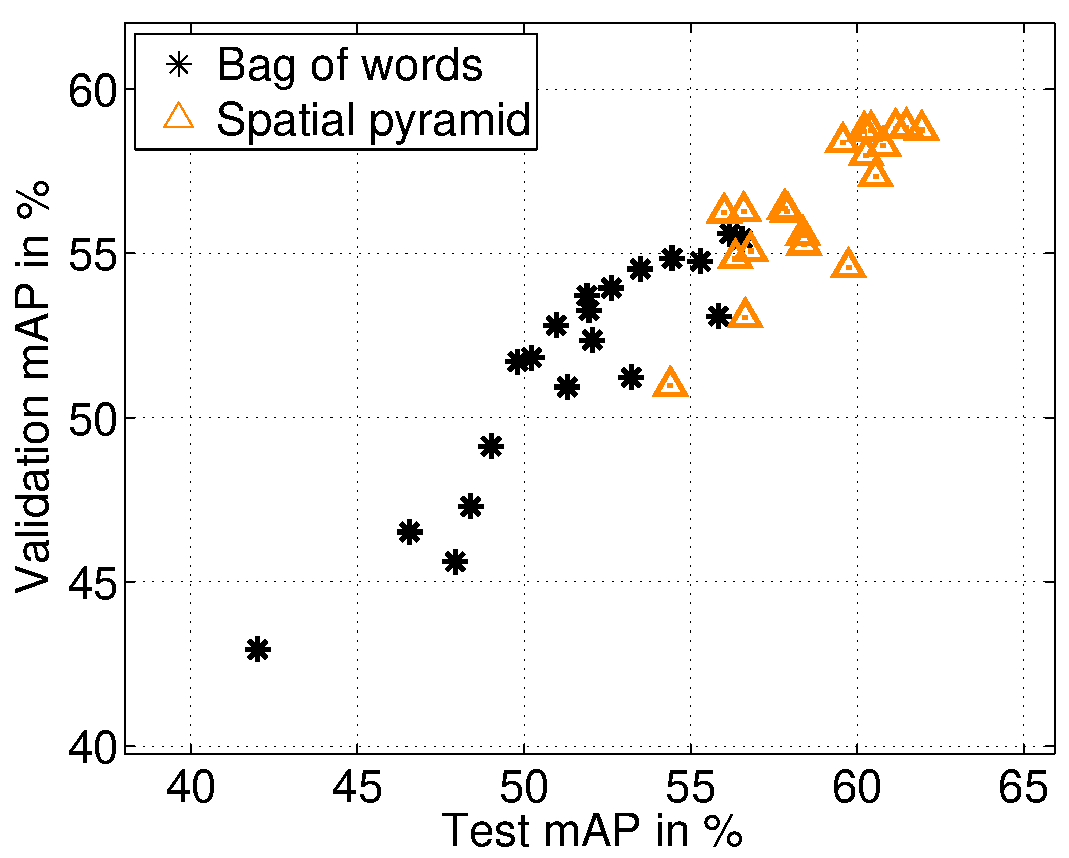
\includegraphics[height=.3\linewidth]{figs/caseA_error_BOF_PYR.pdf} &
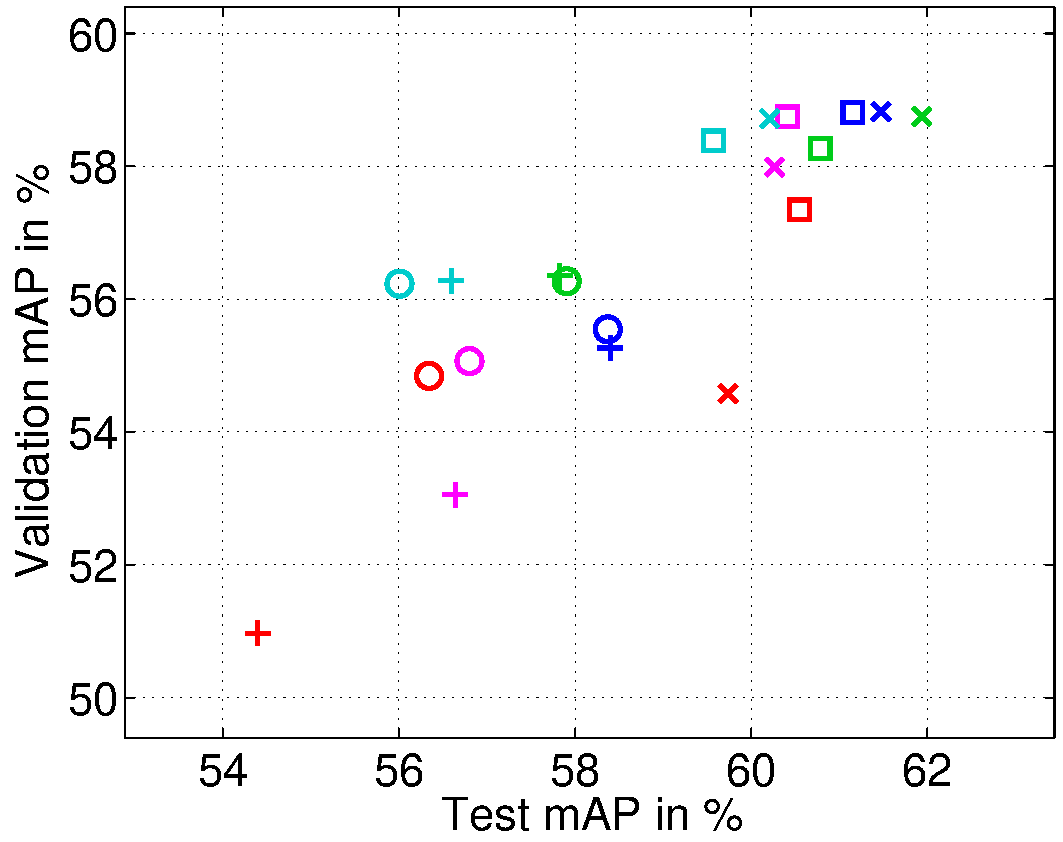
\includegraphics[height=.3\linewidth]{figs/caseA_error_PYR.pdf}
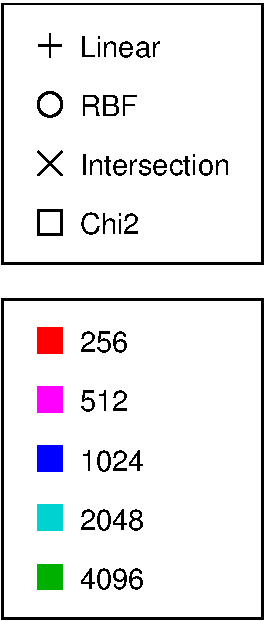
\includegraphics[height=.3\linewidth]{figs/legend.pdf}\\
(a) & (b)  \\
\end{tabular}
\caption{\cfs Classification performance (cross-validation mAP vs. test mAP) for different parameter settings for the BOF method ``A. Person". The best results are at the top right portion of the graph.  (a) Spatial pyramid vs. the bag-of-feature representation.  (b) Classification performance for different combinations of kernels  and vocabulary sizes using the spatial pyramid representation.  Best viewed in color. The  standard deviation (not shown in the plots) of the validation mAP is typically 2-3\%. \normalsize 
}
 \label{fig:caseA}
 \capnspc
\end{figure}



\parnspc
%\paragraph{Is background information beneficial for action classification?}
\paragraph{How to model background context?}
Here we examine the different approaches for incorporating the background information into the bag-of-features action classifier (methods A-C). The overall results are summarized using the classification accuracy and the mean average precision in Table~\ref{tab:methods} (rows A-C2). Classification accuracy across different action classes is shown in Table~\ref{tab:per_class} (columns A-C2).  

Representing the entire image, including the background, with no knowledge about the location of the person (method B) results in a slightly better overall performance than method A where images are cropped to contain only the person performing the action and the background is suppressed.  However, for some actions (``Interacting with computer'' , ``Running" or ``Walking") suppressing the background (method A) is beneficial and reduces their confusion with other classes. %This is likely due to significant variation in the background
%The best overall performance 

The overall performance can be further improved  by treating and matching the foreground and
background separately using two separate kernels (method C2). This holds for all classes except ``Running'' where 
suppressing background (method A) reduces slightly the confusion with the other action classes (and specially ``Walking").
In addition, representing the background with a spatial pyramid (C2) performs better overall than
the vanilla BOF histogram (C1) with no spatial information.
  The overall benefit of treating foreground and background regions separately is inline with the recent experimental evidence
  from object and image classification~\cite{Uijlings09,Zhang07}. 
%In addition, representing the entire image as background with a spatial pyramid (C2) performs better overall than
%representing only the background (non-person) region with BOF histogram (C1).
%The full confusion table for the best performing method (C2) is shown in~\ref{fig:C2_confusion_table}. 
%While accuracy is around 80\% on actions like ``Interacting with computer", ``Riding bike" or ``Walking" other
%actions are more challenging, e.g.: ``Photographing" is often confused with ``Walking" or ``Interacting with Computer", and ``Running" is often confused with ``walking".  These confusions are possibly due to similar human pose or background.

%\red{Vincent, space permitting, show examples of correctly classified results, specially cases  where C2 doing better than.
%to show we learn something about the action not just background. Let's wait with this until LSVM is in.}
%DIscuss the confusions? Space permitting, show correct and misclassified images for each class.\\
%Finally, we note that methods B and C perform better than A, indicating the importance of modelling
%background on our dataset, suggesting 
%Summary is given in table~\ref{tab:methods}(a). \\
%- The whole image (B) (no bounding box info) is better than cropped images (A) (cf. Guptas dataset who has
%cropped images only).\\
%- Describing the whole image with a spatial grid (C2) is better than only the background with BOF (C1).\\
%- B,C1 and C2 are better than A ->  It is beneficial to incorporate background.\\ 

\begin{table}[tbp]
\centering
\rowcolors[]{1}{white}{gray!10}
\begin{tabular}{|l|l||c|c|}
\hline
& \tfs Method                   &\tfs$~~~$mAP$~~~$& \tfs Accuracy  \\ \hline 
\tfs A.   & \tfs BOF Person          & \tfs $61.48$ & \tfs $59.08$ \\ \hline 
\tfs B.   & \tfs BOF Image           & \tfs $62.83$ & \tfs $60.24 $ \\ \hline 
\tfs C1. & \tfs BOF Person+Background& \tfs $63.96$ & \tfs $62.65$ \\ \hline 
\tfs C2. & \tfs BOF Person+Image     & \tfs $70.43$ & \tfs $67.01$ \\ \hline \hline
       & \tfs LSVM              & \tfs $55.12$ & \tfs $57.05$   \\ \hline \hline 
       & \tfs LSVM +  C2    & \tfs ${\bf 72.16}$ & \tfs ${\bf 68.76}$   \\ \hline 
\end{tabular}
\vspace{2mm}
\caption{\cfs The overall classification performance for the different methods. \normalsize}
\label{tab:methods}
\end{table}

\begin{small}
\begin{table}[tbp]
\centering
\rowcolors[]{1}{white}{gray!10}
\begin{tabular}{|l|c|c|c|c||c||c|}
\hline
\tfs Action /  Method & \tfs$~~$A$~~$ & \tfs$~~$B$~~$ & \tfs$~~$C1$~~$ & \tfs$~~$C2$~~$ & \tfs$~~$LSVM$~~$ & \tfs$~$LSVM+C2$~$ \\ \hline 
\tfs(1) Inter. w/ Comp. & \tfs$81.58$ & \tfs$71.05$ & \tfs$71.05$ & \tfs${\bf 84.21}$ & \tfs$42.11$ & \tfs${\bf 84.21}$\\ \hline 
\tfs(2) Photographing   & \tfs$28.95$ & \tfs$28.95$ & \tfs$30.26$ & \tfs${\bf 35.53}$ & \tfs$21.05$ & \tfs$30.26$\\ \hline 
\tfs(3) Playing Music   & \tfs$46.15$ & \tfs$70.09$ & \tfs$70.94$ & \tfs$62.39$ & \tfs${\bf 80.34}$ & \tfs$70.94$\\ \hline 
\tfs(4) Riding Bike     & \tfs$70.21$ & \tfs$73.76$ & \tfs$82.98$ & \tfs$80.85$ & \tfs$63.83$ & \tfs${\bf 84.40}$\\ \hline 
\tfs(5) Riding Horse    & \tfs$50.00$ & \tfs$55.36$ & \tfs$67.86$ & \tfs${\bf 71.43}$ & \tfs$67.86$ & \tfs${\bf 71.43}$\\ \hline 
\tfs(6) Running         & \tfs${\bf 61.25}$ & \tfs$48.75$ & \tfs$40.00$ & \tfs$55.00$ & \tfs$51.25$ & \tfs${\bf 61.25}$\\ \hline 
\tfs(7) Walking         & \tfs$75.42$ & \tfs$73.73$ & \tfs$75.42$ & \tfs${\bf 79.66}$ & \tfs$72.88$ & \tfs$78.81$\\ \hline  \hline
\tfs Average (Accuracy) & \tfs$59.08$ & \tfs$60.24$ & \tfs$62.65$ & \tfs$67.01$ & \tfs$57.05$ & \tfs${\bf 68.76}$\\ \hline 
\end{tabular}
\vspace{2mm}
\caption{\cfs Per-class accuracy across different methods. \normalsize}
\label{tab:per_class}
\tablespc
\end{table}
\end{small}

\parnspc
\paragraph{Part-based model vs. bag-of-features classifier:}
Here we compare the performance of the bag-of-features classification
method (C2),
the structured part-based model (LSVM) and their combination (LSVM+C2).
The overall results are summarized using the classification accuracy
and mean average precision in the last three rows of
Table~\ref{tab:methods}. Classification accuracy across different
action classes is shown in the last three columns of
Table~\ref{tab:per_class}. Interestingly, the part-based model alone
(LSVM) has only limited performance.
The only class where it performs better than the bag-of-features
classifier is ``Playing music".
This might be explained by somewhat consistent set  of human poses for
this action class but fairly varied background.
Overall, the combined LSVM+C2 approach performs best and significantly
improves over the vanilla LSVM.
The improvement of the combined approach over the bag-of-features
classifier (C2) is smaller and depends on the class.
The improvement is largest for action classes ``Riding bike",
``Playing music", ``Riding horse" and ``Running".
For two out of the seven actions the combined approach is actually
slightly worse than C2 alone (Photographing, Walking).
These variations across classes are likely due to the varying levels
of consistency of the human pose (captured well by
structured part-based models), and the overall scene (captured well by
the bag-of-features classifier).
The full confusion table for the overall best performing method
(LSVM+C2) is shown in Table~\ref{tab:confusion_table}.
While accuracy is around 80\% on actions like ``Interacting with
computer", ``Riding bike" or ``Walking" other
actions are more challenging, e.g.: ``Photographing" (accuracy 30\%)
is often confused with ``Walking" or ``Interacting with Computer", and
``Running" (accuracy 61\%) is often confused with ``Walking".
Examples of images correctly classified by the combined LSVM+C2 method
are shown in figures~\ref{fig:corr1} and ~\ref{fig:corr2}.
Examples of challenging images misclassified by the LSVM+C2 method are
shown in figure~\ref{fig:miss2}.
We have found that the combined LSVM+C2 method often improves the
output of  the bag-of-features
 classifier (C2) on images with confusing (blurred, textureless or
unusual) background, but where the pose of the person
is very clear and  the LSVM model provides a confident output.
Similarly, the combined method appears to improve the vanilla LSVM
results mainly in cases where camera viewpoint or the pose of the
person are unusual.

\begin{small}
\begin{table}[tbp]
\centering
\rowcolors[]{1}{white}{gray!10}
\begin{tabular}{|l|c|c|c|c|c|c|c|}
\hline
\tfs Action           & \tfs$~~$(1)$~~$ & \tfs$~~$(2)$~~$ & \tfs$~~$(3)$~~$ & \tfs$~~$(4)$~~$ & \tfs$~~$(5)$~~$ & \tfs$~~$(6)$~~$ & \tfs$~~$(7)$~~$\\ \hline 
\tfs(1) Inter. w/ Comp. & \tfs${\bf 84.21}$ & \tfs$0.00$ & \tfs$15.79$ & \tfs$0.00$ & \tfs$0.00$ & \tfs$0.00$ & \tfs$0.00$\\ \hline 
\tfs(2) Photographing   & \tfs$15.79$ & \tfs${\bf 30.26}$ & \tfs$27.63$ & \tfs$5.26$ & \tfs$0.00$ & \tfs$6.58$ & \tfs$14.47$\\ \hline 
\tfs(3) Playing Music   & \tfs$11.11$ & \tfs$11.11$ & \tfs${\bf 70.94}$ & \tfs$0.85$ & \tfs$2.56$ & \tfs$0.85$ & \tfs$2.56$\\ \hline 
\tfs(4) Riding Bike     & \tfs$0.00$ & \tfs$1.42$ & \tfs$5.67$ & \tfs${\bf 84.40}$ & \tfs$4.26$ & \tfs$0.71$ & \tfs$3.55$\\ \hline 
\tfs(5) Riding Horse    & \tfs$5.36$ & \tfs$3.57$ & \tfs$5.36$ & \tfs$7.14$ & \tfs${\bf 71.43}$ & \tfs$1.79$ & \tfs$5.36$\\ \hline 
\tfs(6) Running         & \tfs$2.50$ & \tfs$5.00$ & \tfs$3.75$ & \tfs$5.00$ & \tfs$0.00$ & \tfs${\bf 61.25}$ & \tfs$22.50$\\ \hline 
\tfs(7) Walking         & \tfs$1.69$ & \tfs$5.08$ & \tfs$3.39$ & \tfs$0.85$ & \tfs$0.85$ & \tfs$9.32$ & \tfs${\bf 78.81}$\\ \hline 

\end{tabular}
\vspace{2mm}
\caption{\cfs Confusion table for the best performing method \green{(LSVM+C2) \normalsize}. 
Accuracy (average of the diagonal): 68.76\%
}
\label{tab:confusion_table}
\tablespc
\end{table}
\end{small}


%\begin{table}[tbp]
%\centering
%\rowcolors[]{1}{white}{gray!10}
%\begin{tabular}{|l|c|c|c|c|c|}
%\hline
%&
%\includegraphics[height=.14\linewidth]{figs/figs/missC2_img0073.png} & 
%\includegraphics[height=.14\linewidth]{figs/figs/missC2_img0073.png} & 
%\includegraphics[height=.14\linewidth]{figs/figs/missC2_img0014.png} & 
%\includegraphics[height=.14\linewidth]{figs/figs/missC2_img0141.png} & 
%\includegraphics[height=.14\linewidth]{figs/figs/missC2_img0057.png}\\ \hline 
%\scriptsize LSVM+C2: & \ok{Walking} & \ok{Walking} & \ok{Running} & \ok{RidingBike} & \ok{PlayingMusic}\\ \hline 
%\scriptsize C2: & \bad{RidingHorse} & \bad{RidingHorse} & \bad{RidingBike} & \bad{Walking} & \bad{Photographing}\\ \hline 
%\end{tabular}
%\caption{\cfs Example images correctly classifier by the combined LSVM+C2 method, but misclassified by the the C2 bag-of-features  approach. \normalsize}
%\end{table}



% \begin{figure}[tbp]
% \centering
% \rowcolors[]{1}{white}{gray!10}
% \begin{tabular}{|c|c|c|c|c|}
% \hline
% \includegraphics[height=.14\linewidth]{figs/figs/misC2_PlayingMusic_instead_RidingHorse_img0062.png} & 
% \includegraphics[height=.14\linewidth]{figs/figs/misC2_Photographing_instead_PlayingMusic_img0160.png} & 
% \includegraphics[height=.14\linewidth]{figs/figs/misC2_RidingHorse_instead_Running_img0037.png} & 
% \includegraphics[height=.14\linewidth]{figs/figs/misC2_InteractingWithComputer_instead_PlayingMusic_img0030} & 
% \includegraphics[height=.14\linewidth]{figs/figs/misC2_InteractingWithComputer_instead_PlayingMusic_img0002.png}\\ \hline 
% \scriptsize LSVM+C2: ~ \ok{RidingHorse} &  \ok{PlayingMusic} & \ok{Running} & \ok{\scriptsize Play. Music} & \ok{Play. Music}\\ \hline 
% \scriptsize C2: ~\bad{PlayingMusic} &\bad{Photograping}  & \bad{RidingHorse} & \bad{\scriptsize In. w/ comp.} & \bad{\scriptsize In. w/ comp.}\\ \hline 
% \end{tabular}
% \caption{\cfs Example images correctly classified by the combined LSVM+C2 method (labels on the 2nd row), but misclassified by the C2 bag-of-features  approach (labels on the 3rd row). \normalsize}
% \label{fig:corr1}
% \capnspc
% \end{figure}
% 
% \begin{figure}[tbp]
% \centering
% \rowcolors[]{1}{white}{gray!10}
% \begin{tabular}{|c|c|c|c|c|}
% \hline
% \includegraphics[height=.14\linewidth]{figs/figs/misLSVM_PlayingMusic_instead_Photographing_img0009.png} & 
% \includegraphics[height=.14\linewidth]{figs/figs/misLSVM_PlayingMusic_instead_RidingBike_img0032.png} & 
% \includegraphics[height=.14\linewidth]{figs/figs/misLSVM_PlayingMusic_instead_RidingHorse_img0032.png} & 
% \includegraphics[height=.14\linewidth]{figs/figs/misLSVM_RidingHorse_instead_RidingBike_img0192.png} & 
% \includegraphics[height=.14\linewidth]{figs/figs/misLSVM_Running_instead_Photographing_img0114.png}\\ \hline 
% \scriptsize LSVM+C2: \ok{Photographing} & \ok{RidingBike} & \ok{RidingHorse} & \ok{ RidingBike} & \ok{Photograph.}\\ \hline 
% \scriptsize LSVM: \bad{PlayingMusic} & \bad{PlayingMusic} & \bad{PlayingMusic} & \bad{RidingHorse} & \bad{Running}\\ \hline 
% \end{tabular}
% \caption{\cfs Example images correctly classified by the combined LSVM+C2 method (labels on the 2nd row), but misclassified by the part-based LSVM  approach (labels on the 3rd row). \normalsize}
% \label{fig:corr2}
% \capnspc
% \end{figure}
% 
% \begin{figure}[tbp]
% \centering
% \rowcolors[]{1}{white}{gray!10}
% \begin{tabular}{|c|c|c|c|c|}
% \hline
% \includegraphics[height=.14\linewidth]{figs/figs/misLSVMC2_InteractingWithComputer_instead_PlayingMusic_img0154.png} & 
% \includegraphics[height=.14\linewidth]{figs/figs/misLSVMC2_Walking_instead_Photographing_img0117.png} & 
% \includegraphics[height=.14\linewidth]{figs/figs/misLSVMC2_RidingBike_instead_RidingHorse_img0125.png} & 
% \includegraphics[height=.14\linewidth]{figs/figs/misLSVMC2_Running_instead_Walking_img0060.png} & 
% 
\includegraphics[height=.14\linewidth]{figs/figs/misLSVMC2_PlayingMusic_instead_InteractingWithComputer_img0036.png}\\ \hline 
%  \scriptsize LSVM+C2: \bad{Inter. w/ comp.} & \bad{Walking} & \bad{RidingBike} & \bad{Running} & \bad{PlayingMusic}\\ \hline 
%  \scriptsize G.T.: \ok{PlayingMusic} & \ok{Photographing} & \ok{RidingHorse} & \ok{Walking} & \ok{Inter. w/ comp.}\\ \hline 
% \end{tabular}
% 
% \caption{\cfs Examples of challenging images misclassified by the combined LSVM+C2 method (labels on the 2nd row). The ground truth labels are shown in the 3rd row.  Note the variation in viewpoint, scale, partial occlusion. \normalsize}
% \label{fig:miss2}
% \capnspc
% \end{figure}


%
%\begin{table}[H]
%\centering
%\rowcolors[]{1}{white}{gray!10}\begin{tabular}{|c|c|c|c|c|}
%\hline
%Images & \includegraphics[height=2cm]{figs/missLSVM_img0032.png} & \includegraphics[height=2cm]{figs/missLSVM_img0009.png} & \includegraphics[height=2cm]{figs/missLSVM_img0028.png} & \includegraphics[height=2cm]{figs/missLSVM_img0035.png}\\ \hline 
%Correct label & RidingBike & Photographing & RidingBike & RidingHorse\\ \hline 
%Result label & PlayingMusic & PlayingMusic & Photographing & Walking\\ \hline 
%\end{tabular}
%\caption{\cfs Missclassified by LSVM but not LSVM+C2 \normalsize}
%\end{table}

%\begin{table}[H]
%\centering
%\rowcolors[]{1}{white}{gray!10}\begin{tabular}{|c|c|c|c|c|}
%\hline
%Images & \includegraphics[height=2cm]{figs/missLSVMC2_img0071.png} & \includegraphics[height=2cm]{figs/missLSVMC2_img0132.png} & \includegraphics[height=2cm]{figs/missLSVMC2_img0180.png} & \includegraphics[height=2cm]{figs/missLSVMC2_img0113.png}\\ \hline 
%Correct label & Photographing & Photographing & PlayingMusic & PlayingMusic\\ \hline 
%Result label & PlayingMusic & InteractingWithComputer & InteractingWithComputer & Photographing\\ \hline 
%\end{tabular}
%\caption{\cfs Missclassified by LSVM+C2 \normalsize}
%\end{table}



\parnspc
%\paragraph{Comparison on the sports dataset of Gupta~\etal~\cite{Gupta09}:} 
%Results are shown in table~\ref{tab:methods}(b).
%As shown in table~\ref{tab:gupta}(b), our approach outperforms the approach of Gupta~\etal by more than 6\%.
%We have cross-validated again the parameters of the bag-of-features classifier and found that  bigger vocabularies ($K=4096$) perform
%better on this dataset. Other parameters (the intersection kernel, and spatial pyramid binning) remain the same. 
%Note that the approach of Gupta~\etal uses the location of people and the surrounding objects in training. 
%In our method, no person bounding box information is used in training or test. However, as the images in the original dataset
%are already cropped and centered to contain mostly the person of interest the approach is comparable with method A on our dataset. 

\begin{figure}[ht]
\centering
\rowcolors[]{1}{white}{gray!10}
\begin{tabular}{|c|c|c|c|c|}
\hline
\includegraphics[height=.14\linewidth]{figs/misC2_PlayingMusic_instead_RidingHorse_img0062.png}
&
\includegraphics[height=.14\linewidth]{figs/misC2_Photographing_instead_PlayingMusic_img0160.png}
&
\includegraphics[height=.14\linewidth]{figs/misC2_RidingHorse_instead_Running_img0037.png}
&
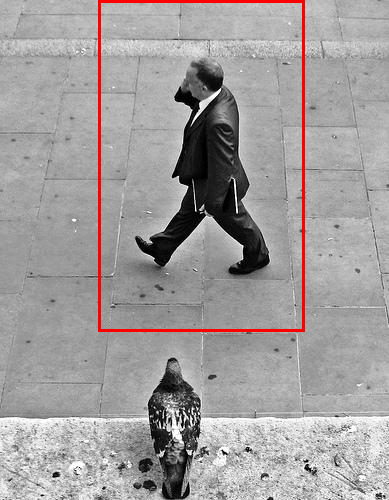
\includegraphics[height=.14\linewidth]{figs/misC2_RidingHorse_instead_Walking_img0073.png}
&
\includegraphics[height=.14\linewidth]{figs/misC2_InteractingWithComputer_instead_PlayingMusic_img0002.png}\\
\hline
\scriptsize LSVM+C2: | ~ \ok{RidingHorse} &  \ok{PlayingMusic} &
\ok{Running} & \ok{\scriptsize Walking} & \ok{Play. Music}\\ \hline
\scriptsize C2: | ~\bad{PlayingMusic} &\bad{Photograping}  &
\bad{RidingHorse} & \bad{\scriptsize RidingHorse} & \bad{\scriptsize
In. w/ comp.}\\ \hline
\end{tabular}
\vspace{2mm}
\caption{\cfs Example images correctly classified by the combined LSVM+C2
method (labels in the 2nd row), but misclassified by the C2
bag-of-features  approach (labels in the 3rd row). \normalsize}
\label{fig:corr1}
\capnspc
\end{figure}

\begin{figure}[ht]
\centering
\rowcolors[]{1}{white}{gray!10}
\begin{tabular}{|c|c|c|c|c|}
\hline
\includegraphics[height=.14\linewidth]{figs/misLSVM_PlayingMusic_instead_Photographing_img0009.png}
&
\includegraphics[height=.14\linewidth]{figs/misLSVM_PlayingMusic_instead_RidingBike_img0032.png}
&
\includegraphics[height=.14\linewidth]{figs/misLSVM_PlayingMusic_instead_RidingHorse_img0032.png}
&
\includegraphics[height=.14\linewidth]{figs/misLSVM_RidingHorse_instead_RidingBike_img0192.png}
&
\includegraphics[height=.14\linewidth]{figs/misLSVM_Running_instead_Photographing_img0114.png}\\
\hline
\scriptsize LSVM+C2: |  \ok{Photographing} & \ok{RidingBike} &
\ok{RidingHorse} & \ok{ RidingBike} & \ok{Photograph.}\\ \hline
\scriptsize LSVM:  | ~~~\bad{PlayingMusic} & \bad{PlayingMusic} &
\bad{PlayingMusic} & \bad{RidingHorse} & \bad{Running}\\ \hline
\end{tabular}
\vspace{2mm}
\caption{\cfs Example images correctly classified by the combined LSVM+C2
method (labels in the 2nd row), but misclassified by the part-based
LSVM  approach (labels in the 3rd row). \normalsize}
\label{fig:corr2}
\capnspc
\end{figure}

\begin{figure}[ht]
\centering
\rowcolors[]{1}{white}{gray!10}
\begin{tabular}{|c|c|c|c|c|}
\hline
\includegraphics[height=.14\linewidth]{figs/misLSVMC2_InteractingWithComputer_instead_PlayingMusic_img0154.png}
&
\includegraphics[height=.14\linewidth]{figs/misLSVMC2_Walking_instead_Photographing_img0117.png}
&
\includegraphics[height=.14\linewidth]{figs/misLSVMC2_RidingBike_instead_RidingHorse_img0125.png}
&
\includegraphics[height=.14\linewidth]{figs/misLSVMC2_Running_instead_Walking_img0060.png}
&

\includegraphics[height=.14\linewidth]{figs/misLSVMC2_PlayingMusic_instead_InteractingWithComputer_img0036.png}\\
\hline
 \scriptsize LSVM+C2: | \bad{Inter. w/ comp.} & \bad{Walking} &
\bad{RidingBike} & \bad{Running} & \bad{PlayingMusic}\\ \hline
 \scriptsize G.T.: | ~~~\ok{PlayingMusic} & \ok{Photographing} &
\ok{RidingHorse} & \ok{Walking} & \ok{Inter. w/ comp.}\\ \hline
\end{tabular}
%\vspace{1mm}
\caption{\cfs Examples of challenging images misclassified by the combined
LSVM+C2 method (labels in the 2nd row). The ground truth labels are
shown in the 3rd row.  Note the variation in viewpoint, scale, partial
occlusion. \normalsize}
\label{fig:miss2}
\capnspc
\end{figure}

%\paragraph{Comparison on the sports dataset of Gupta~\etal~\cite{Gupta09}:}
%As shown in table~\ref{tab:gupta}, both the BOF and LSVM+BOF methods
%outperform the approach of Gupta~\etal by more than 6\%. We have
%cross-validated again the parameters of the bag-of-features classifier
%and found that  bigger vocabularies ($K=4096$) perform better on this
%dataset. Other parameters (the intersection kernel, and spatial
%pyramid binning) remain the same.
%The vanilla LSVM model has again lower overall classification
%performance than the BOF classifier.
%By examining the results, we have found that the LSVM model mainly
%confuses the ``Tennis serve" and ``Volleyball smash" actions, possibly
%due to the similarity of the (vertically extended) human pose. On the
%other hand, the bag-of-features classifier can still distinguish the
%two classes fairly well. Furthermore, the combined LSVM+BOF approach
%reaches, and marginally outperforms, the bag-of-features classifier.
%Note that the approach of Gupta~\etal uses the location of people and
%the surrounding objects in training.
%In our method, no person bounding box information is used in training
%or test. However, as the images in the original dataset
%are already cropped and centered to contain mostly the person of
%interest the approach is comparable with method A on our dataset.

\paragraph{Comparison with the state of the art~\cite{Gupta09,FeiFei10a, FeiFei10b}:}
For both datasetst~\cite{Gupta09,FeiFei10a}, no person bounding box information is used neither in training
nor in test (method B). However, as the images in the original dataset
are already cropped and centered to contain mostly the person of
interest, the approach is comparable with method A on our dataset.
For the sport dataset of Gupta~\etal~\cite{Gupta09} we have
cross-validated again the parameters of the bag-of-features classifier
and found that larger vocabularies ($K=4096$) perform better on this
dataset. Other parameters (the intersection kernel and spatial
pyramid binning) remain the same.
For the Person Playing Musical Instrument dataset of Yao and Fei-Fei ~\cite{FeiFei10a}
we adopted a denser sampling of the SIFT features with initial spacing of 6 pixels to adapt
to the smaller size of the images. Moreover we used a 3 level spatial pyramid and a LSVM
with 9 parts to have a denser spatial coverage. Other parameters (the intersection kernel 
and $K=1024$) remain the same.
As shown in Table~\ref{tab:StateOfArt}, both the BOF and LSVM+BOF methods
outperform the approach of Gupta~\etal and Yao and Fei-Fei by 1.7\% to 9.4\%.



\begin{table}[t]
\centering
\rowcolors[]{1}{white}{gray!10}
\begin{tabular}{|l||c|c||c|c|c|c|}
\hline
                        & \multicolumn{2}{c||}{\multirow{2}*{Gupta et al.}}  &\multicolumn{4}{c|}{Yao and Fei-Fei \cite{FeiFei10a}}     \\ \cline{4-7}
\multirow{-2}*{Dataset} & \multicolumn{2}{c||}{}                             &\multicolumn{2}{c|}{Task 1} &\multicolumn{2}{c|}{Task 2}  \\ \hline
Method  			                               & mAP             & Acc.           & mAP               & Acc.         & mAP               & Acc.                \\ \hline \hline
Gupta~\etal~~\cite{Gupta09}	                 & --         	   & $78.7$         & --                & --           & --                & --                  \\ \hline 
Yao and Fei-Fei~~\cite{FeiFei10a, FeiFei10b} & --	             & $83.3$         & --                & $65.7$       & --                & $80.9$              \\ \hline 
BOF Image (B) 		 	                         & $91.3$	         & ${\bf 85.0}$   & $76.9$            & $71.7$       & $87.7$            & $83.7$              \\ \hline 
LSVM 			  		                             & $77.2$          & $ 73.3 $       & $53.6$            & $67.6$       & $82.2$            & $82.9$              \\ \hline 
LSVM + BOF Image (B)		                     & ${\bf 91.6}$    & $ {\bf 85.0}$  & ${\bf 77.8}$      & ${\bf 75.1}$ & ${\bf 90.5}$      & ${\bf 84.9}$        \\ \hline 
\end{tabular}
\vspace{2mm}
\caption{\cfs Comparison with the method of Gupta~\etal.~\cite{Gupta09} and of Yao and Fei-Fei \cite{FeiFei10a, FeiFei10b} on their datasets. `Task 1' is the 7-class
classification problem and `Task 2' is the PPMI+ vs PPMI- problem (see \cite{FeiFei10a}).\normalsize}
\label{tab:StateOfArt}
\tablespc
\end{table}


%%%%%%%%%%%%%%%%%%%%%%%%
\secnspc
\section{Conclusions}
\secnspc
%%%%%%%%%%%%%%%%%%%%%%%%

%We have collected a new challenging dataset of more than 900 consumer photographs depicting seven 
%common human actions. 
We have studied the performance of the bag-of-features classifier and the latent SVM
model~\cite{Felzenszwalb09} on the task of action recognition in still images.
We have collected a new challenging dataset of more than 900 consumer photographs depicting seven everyday human actions.
We have demonstrated on this data, as well as on two existing datasets of person-object interactions~\cite{Gupta09,FeiFei10a},  that  (i) combining statistical and structured part-based representations and (ii) incorporating scene background context can lead to significant improvements in action recognition performance in still images. 
Currently, almost all tested methods (except the image-level classifier B) use the manually provided person bounding boxes. 
Next, we plan to investigate incorporating real person detections~\cite{Dalal05,Felzenszwalb09} into the classifier.



\paragraph{Acknowledgements:}  
We are grateful for financial support 
from the MSR-INRIA laboratory and the Quaero Programme, funded by OSEO.
 

%
%Except method B, all methods rely on knowing the rough location of the person performing the action
%in the image, which is provided manually.
%The best performing methods (C2 and LSVM+C2) are trained from the rough location of the person performing
%the action in the image. 
%classifier relies on a coarse localization
%We have investigated statistical bag-of-features and structured part-based representations
%for action recognition in still images and demonstrated that their combination
%can improve classification performance. 

 

%We have addressed the relatively unexplored problem of action recognition in still images.
%
%While action recognition in video has recently received significant attention, action recognition
%in still images is relatively unexplored domain. 
%%- We address the problem of action recognition in still images.
%Following contributions:
%- investigate the bof representation on the problem.  
%Experimentaly compare a range of parameters including kernels, and different ways of including background information and show that representation combining of person centric description and image level description on the kernel level performs best. \\
%- further show that combining with structured discrimintively trained flexible part based person centric representation of Felzenswalb et al. further improves performance. \\
%- collect new dataset of real Flickr images containing common everyday actions  not focused on a particular domain such as  sports.\\
%- Show results on the newly collected dataset. outperform the approach of Gupta on his own dataset. 


\bibliography{shortstrings,paper}
\end{document}
